\documentclass[acmsmall,nonacm]{acmart}

\usepackage{tikz}
\usetikzlibrary{positioning, fit, shapes, arrows}
\usepackage{float}

\begin{document}

\title{From Structural Mapping to Intention Reasoning: A Review of LLM-based Mobile Test Migration}

\author{Tian Gan}
\email{tian.gan@tum.de}
\affiliation{\institution{Technical University of Munich}\country{Germany}}

\begin{abstract}
Testing mobile applications across users' devices remains challenging due to ecosystem fragmentation and the brittleness of UI-dependent automation techniques. Traditional test migration approaches rely heavily on static UI attributes, such as XML resource identifiers. Those limits their robustness across structurally dissimilar applications. 

This report argues how recent Large Language Model (LLM)–based approaches address this limitation by shifting test migration from structure-level mapping to intention-level reasoning. By synthesizing recent literature, I broken the process down into a three-stage pipeline: abstraction of test intent, planning of execution, and finally grounding actions back to concrete UI elements. 

Although LLM-based frameworks do solve the limits to some extent, demonstrating improved flexibility and cross-app adaptability. But through analysis, the report unearths persistent challenges, likewise hallucination, visual grounding errors, and execution instability. In the end, this report discusses the present industrial application, such as applications at Amazon. And it argues that mixed approaches combine LLM reasoning with traditional verification mechanisms which shows potential for reliable large-scale deployment.
\end{abstract}

\keywords{Mobile App Testing, Large Language Model, Automated Test Migration}

\maketitle

\section{Introduction}
Developing for the device ecosystem is often a struggle against sheer fragmentation, as apps must operate across various screen dimensions, OS versions, and hardware specs. While the testers rely on the automated GUI testing to catch bugs, the reality is that maintaining these tests is a expensive and time-consuming burden. The core problem is the inherent brittleness. Even a minor UI in enough to break a test scripts, forcing developers suffering from manual repairs and rewrites  \cite{10.1145/3236024.3236055,8952228}.

To lower long-term maintenance cost, previous researchers have focused on reusing or transferring test cases and logic from one application to another. The two applications share similar functionality \cite{8952228,10.1145/3650212.3680327}. Most traditional approaches depend on UI features, such as XML resource identifiers, widget hierarchies, or predefined semantic mappings between screens \cite{10.1145/3236024.3236055,8952228}. Although these strategies work well in controlled experiments, they often break down on real-world applications, because of the diverse workflows, dynamic content, or non-standard UI layouts \cite{8952228,10.1145/3650212.3680327}. As a result, test migration remains brittle when structural similarity between source and target applications is limited.

Recently, Large Language Models (LLMs) have begun to offer another way to help overcome these shortcomings \cite{10.1145/3728975,10.1145/3728978,10.1145/3236024.3236055,zhang2024surveylargelanguagemodels}. Rather than primarily relying on structural correspondences, LLM-based approaches attempt to reason about the intention behind a test cas. For example, confirming a successful login or adding an item to a shopping cart, and then mapping this intention to a new application environment \cite{10.1145/3728975,10.1145/3728978,10.1145/3726525}. By their ability to capture and abstract semantic relationships and procedural logic, LLMs transfer the focus from brittle, structural level mapping to more flexible, intention level reasoning \cite{10.1145/3728975,10.1145/3236024.3236055,zhang2024surveylargelanguagemodels}.

However, adopting LLMs can not solve all problems. Though recent frameworks demonstrate higher flexibility, they introduce new sources of uncertainty \cite{li2025reusedroidvlmempoweredandroidui,wang2024softwaretestinglargelanguage}. Issues such as hallucinated actions, incorrect visual grounding, and unstable execution behavior have been repeatedly reported in the literature \cite{baechler2024screenaivisionlanguagemodelui,li2025reusedroidvlmempoweredandroidui,wang2024softwaretestinglargelanguage,zhang2025largelanguagemodelbrainedgui}. And some researchers pointed out that in their experiments LLMs can not reach the success rates as expected and exhibited in previous literature. These limitations raise important questions about the reliability, scalability, and practical deployment of LLM-based systems.

This subsequent report is organized into five sections. Section 2 begins by establishing the background on automated mobile application testing and reviewing two mainstream pre-LLMs approaches. Then the report analyzes recent LLM-based test migration frameworks and visualizes the workflow into a three-step abstraction–planning–grounding pipeline in Section 3. Section 4 discusses the key challenges and open problems associated with LLM-driven migration, including semantic drift, visual grounding errors, and evaluation limitations. To bridge the gap between academic theory and industrial applications, Section 5 then explores future directions and examines emerging industrial practices. It looks at how Amazon handle large-scale deployment scenarios. Finally, the report wraps up in Section 6 with a summary of concluding thoughts.



\section{Background}

\subsection{Pre-LLMs Approaches}
Prior to the emergence of Large Language Models, automated test migration primarily relied on heuristic rules and static analysis. These approaches can be broadly categorized into \textbf{Mapping-based} \cite{li2025reusedroidvlmempoweredandroidui} and \textbf{Search-and-Synthesis-based} methods \cite{10.1145/3650212.3680327}.

\begin{itemize}
    \item \textbf{Mapping-based Approach:} Represented by frameworks like \textbf{CraftDroid}, this category focuses on transferring test cases and oracle through semantic mapping. \textbf{CraftDroid} operates via a three-component pipeline \cite{8952228}:
    \begin{itemize}
        \item\textbf{Test Augmentation} instruments the source app, augments the original test cases to extract textual information from the exercised GUI widgets.
        \item\textbf{Model Extraction} employs static analysis on the target app to map transitions between Activity components, constructing a UI Transition Graph (UITG).
        \item\textbf{Test Generation} calculates the similarity between source and target widgets. It uses textual information and location of widgets in the UITG. The calculation relies on NLP token matching and a (Word2Vec)-based weighting algorithm. Finally it generates new tests, transfers oracles (including negative checks) and verifies path reachability on the target app.
    \end{itemize}
    
    While this architecture proved effective for applications with simple textual correspondence , it suffers from a lack of contextual understanding. Because the method processes widgets in isolation, it fails to capture the sequential logic inherent in complex test scenarios. Consequently, the mapping mechanism often breaks when target applications employ textless icons or divergent workflows. Furthermore, the over-reliance on static UITG performs poorly on complex and large-size apps. For instance, transfer success rates drop significantly in complex domains such as shopping applications \cite{8952228}.

    
    \item \textbf{Search-and-Synthesis-based Approach:} Conversely, frameworks like \textbf{Appflow} utilize supervised machine learning to explore the application's state space rather than relying on direct mapping. By recognizing screens and widgets, it synthesizes tests through traversing a pre-defined behavior graph. This methodology is primarily structured into two phases \cite{10.1145/3236024.3236055}: \begin{enumerate}
        \item \textbf{Offline Learning: }It utilizes large-scale labeled datasets to train deep learning classifiers. By analyzing large-scale dataset of GUI screenshots and layout information, it identifies common abstract screens and abstract widgets. This effectively decouples test execution from underlying resource IDs.
        \item \textbf{Online Synthesis: }Via traversing a pre-defined Behavior Graph that describes the states of screens and actions, it dynamically maps abstract user paths to concrete widgets on the current screen, guiding the exploration of the application's state space.
    \end{enumerate}

    Although AppFlow demonstrated strong resilience to UI layout changes and fragile resource IDs, it remains limited by its inability to understand test intent. Critical drawbacks include \cite{8952228} \begin{enumerate}\item a Lack of context-awareness in inputs; \item Limited expressiveness in test generation. \item Absence of oracles. \end{enumerate} Moreover, the heavy reliance on supervised learning restricts domain generalization. The approach is often confined to specific app categories and cannot adapt to new genres without retraining on extensive datasets.
    \end{itemize}

\subsection{Overview of LLM}
LLMs have recently become an important foundation for software engineering tasks involving code understanding and transformation. Trained on large-scale corpora of natural language and source code, LLMs are able to capture both syntactic structures and higher-level semantic relationships between code elements\cite{zhang2024surveylargelanguagemodels}. This property is particularly relevant to automated test script migration, where preserving test intent and execution logic across heterogeneous mobile applications is a central challenge.

From a task-oriented perspective, automated test script migration can be viewed as a sequence-to-sequence transformation problem: a source test script encodes a sequence of user actions and assertions, while the target script aims to reproduce equivalent functionality under different UI structures, identifiers, or workflows. Previous migration approaches rely heavily on manually engineered abstractions or similarity heuristics, which limits their robustness and generalization ability \cite{10.1145/3236024.3236055,8952228}. In contrast, LLMs provide a data-driven alternative by learning implicit correspondences between code, textual context, and execution semantics directly from training data.

According to recent surveys on LLMs for software engineering, two capabilities are particularly relevant to test script migration: code generation and code translation \cite{zhang2024surveylargelanguagemodels}. Code generation enables LLMs to synthesize executable test scripts in a target framework while adapting API calls, UI locators, and control structures. Code translation allows LLMs to transform existing scripts across applications or testing environments while preserving functional intent, even when UI hierarchies and resource identifiers differ substantially. Compared to traditional AST-based techniques, these capabilities operate at a semantic level and are better suited to handling dynamic identifiers and structurally dissimilar interfaces \cite{zhang2024surveylargelanguagemodels}.


Overall, the integration of LLMs shifts test script migration from manually designed abstraction rules toward intent-aware adaptation. While this introduces new challenges such as controllability and reproducibility, recent work suggests that LLM-based approaches can reduce manual effort and improve the maintainability of migrated test scripts when combined with appropriate validation mechanisms \cite{zhang2024surveylargelanguagemodels}.



\section{Methodology}

\subsection{Methodological Framework Overview}
From a methodological perspective, the integration of Large Language Models (LLMs) into test migration represents more than just a technical upgrade; it marks a fundamental paradigm shift from structure-level mapping to intention-level reasoning. Unlike traditional approaches that relied heavily on rigid heuristic rules \cite{8952228}, modern frameworks operate by decoupling the abstract test intention from its concrete implementation. While architectural choices vary across recent studies—such as \textbf{LLMigrate} \cite{10.1145/3728975}, \textbf{ReuseDroid} \cite{li2025reusedroidvlmempoweredandroidui}, and \textbf{MigratePro}—the general methodology converges into a three-stage pipeline: Abstraction, Planning, and Grounding.As illustrated in Fig. 1, this pipeline provides a conceptual overview of how source test traces are transformed into executable actions on heterogeneous target UIs through intention reasoning and visual grounding.


\begin{figure}[H] 
    \centering
    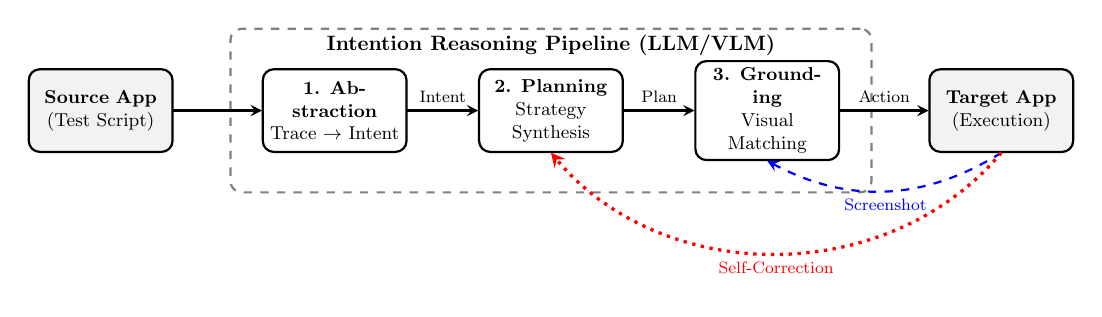
\begin{tikzpicture}[node distance=1.5cm, auto, >=stealth, scale=0.75, transform shape]
        \tikzstyle{box} = [rectangle, draw=black, thick, fill=gray!10, text width=2.2cm, text centered, rounded corners, minimum height=1.4cm, font=\small]
        \tikzstyle{llm_box} = [rectangle, draw=black, thick, fill=white, text width=2.2cm, text centered, rounded corners, minimum height=1.4cm, font=\small]
        \tikzstyle{container} = [draw=gray, dashed, thick, inner sep=0.4cm, rounded corners, label={[anchor=north]north:{\textbf{Intention Reasoning Pipeline (LLM/VLM)}}}]

        \node [box] (source) {\textbf{Source App} \\ (Test Script)};
        
        \node [llm_box, right=1.5cm of source] (abs) {\textbf{1. Abstraction} \\ Trace $\to$ Intent};
        \node [llm_box, right=1.2cm of abs] (plan) {\textbf{2. Planning} \\ Strategy Synthesis};
        \node [llm_box, right=1.2cm of plan] (ground) {\textbf{3. Grounding} \\ Visual Matching};
        
        \node [box, right=1.5cm of ground] (target) {\textbf{Target App} \\ (Execution)};

        \node [container, fit=(abs) (plan) (ground)] (pipeline) {};

        \draw [->, thick] (source) -- (abs);
        \draw [->, thick] (abs) -- node[above, font=\footnotesize] {Intent} (plan);
        \draw [->, thick] (plan) -- node[above, font=\footnotesize] {Plan} (ground);
        \draw [->, thick] (ground) -- node[above, font=\footnotesize] {Action} (target);

        \draw [->, dashed, blue, thick] (target.south) to[bend left=30] node[below, font=\footnotesize] {Screenshot} (ground.south);
        \draw [->, dotted, red, very thick] (target.south) to[bend left=50] node[below, font=\footnotesize] {Self-Correction} (plan.south);

    \end{tikzpicture}
    \caption{Conceptual abstraction of LLM-driven test migration pipelines. The workflow summarizes recurring components reported in prior work, emphasizing intent reasoning, planning, and visual grounding, together with feedback loops commonly adopted for adaptive execution.}
    \label{fig:workflow}
\end{figure}

\begin{itemize}
    \item Step 1: \textbf{Comprehension and Abstraction:
    }
    
    A major hurdle in test migration lies in the significant structural divergence between source and target applications, such as differing XML hierarchies and resource IDs. To address this, current frameworks typically leverage LLMs to transform low-level execution traces into a platform-agnostic Intermediate Representation (IR). For instance, \textbf{ITEM} \cite{10.1145/3728978} summarizes these traces into natural language intentions (e.g., "Search for product 'X'"), while \textbf{MACdroid} \cite{10.1145/3726525} attempts to mitigate bias by extracting a "General Test Logic" derived from multiple apps.

    However, using natural language as an IR is not without risks. It introduces a layer of ambiguity, as the same intention description might be interpreted differently by downstream planners, especially when domain-specific constraints are implicit rather than explicit. Consequently, the quality of abstraction in this initial stage effectively sets the upper bound for the success of the entire migration process.

    
    \item Step 2: \textbf{Planning and Reasoning: } 
    
    Once an abstract intention is formulated, the system faces the challenge of bridging the semantic gap to the unseen target UI. This stage necessitates complex reasoning, particularly to resolve the \textbf{1-to-N mapping problem}, where a single abstract step like "Login" might require a multi-step interaction sequence in the target app due to workflow discrepancies.

    Approaches in the literature differ significantly here. \textbf{ReuseDroid} \cite{li2025reusedroidvlmempoweredandroidui} utilizes a Planner Agent to decompose high-level goals into atomic actions based on the current UI state. In contrast, \textbf{MigratePro} adopts a synthesis-based approach, building a State Graph to explore and generate entirely new paths. From a critical standpoint, this highlights a fundamental trade-off: while planner-based approaches tend to preserve the original test semantics more faithfully, synthesis-based approaches appear to offer higher adaptability across structurally dissimilar apps, albeit at the cost of potential deviation from the original test scenario.

    \item Step 3: \textbf{Visual Grounding and Execution: }
    
    The final stage involves Visual Grounding, where abstract plans are anchored to concrete UI elements. To mitigate the "Hallucination vs. Reality" gap—especially when accessibility metadata is missing—frameworks like \textbf{ScreenAI} \cite{baechler2024screenaivisionlanguagemodelui} integrate Vision-Language Models (VLMs) to identify elements based on visual features.
    
    In practice, this stage arguably represents the most fragile link in the pipeline. Unlike planning errors, which can often be recovered through re-reasoning, grounding errors (such as false positive element detection) are harder to detect and can silently invalidate the test execution. Furthermore, the non-deterministic nature of VLM outputs introduces a degree of instability that remains a significant challenge for industrial adoption.
\end{itemize}

\subsection{Enabling Technologies and Trade-offs}
To support this open-ended reasoning process, several technical components are essential, though they each introduce specific limitations.

\textbf{Prompt Engineering and Context Limits.} Techniques such as \textbf{In-Context Learning} and \textbf{Chain-of-Thought (CoT)} \cite{wei2023chainofthoughtpromptingelicitsreasoning} are widely employed to bridge the cognitive gap between human intent and machine execution. However, these strategies are inevitably bounded by the Context Window Limit. Including extensive UI hierarchy data and few-shot examples often exhausts the token budget, which may force a trade-off between the depth of context provided and the complexity of the reasoning required.

\textbf{Multimodal Context Management.} While feeding screenshots directly to Multimodal LLMs compensates for the lack of reliable text attributes, it incurs significant computational costs. Moreover, the necessity of resizing high-resolution screenshots to fit model constraints can lead to the loss of fine-grained visual details, making it difficult for the model to interact with smaller UI elements.

\textbf{Self-Correction Loops.} Frameworks like \textbf{LLMigrate} \cite{10.1145/3728975} attempt to mitigate these issues by implementing feedback loops where execution errors trigger re-planning. While this significantly improves robustness compared to static scripts, it is not a panacea; from the reported results, it appears that systems can still fall into infinite correction loops if the underlying reasoning logic is fundamentally flawed.

\textbf{Summary:} Together, these components enable LLM-based migration frameworks to operate in dynamic, open-ended GUI environments. However, they also shift the primary challenge from manual script maintenance to managing the efficiency, robustness, and stochastic nature of AI-driven agents.

\section{Challenges and Open Problems}
Despite the promising methodology outlined in Section 3, recent LLM-based test migration frameworks continue to face fundamental challenges that limit their robustness, scalability, and practical applicability. Importantly, these challenges are not isolated to individual components but emerge across the abstraction–planning–grounding pipeline, as consistently reported in both method-driven studies and recent survey work.

\subsection{Ambiguity and Semantic Drift in Intention Abstraction}
A core challenge arises during the abstraction stage, where low-level test scripts are transformed into intention-level representations. Approaches such as \textbf{MACdroid} \cite{10.1145/3726525} and \textbf{ITEM} \cite{10.1145/3728978} demonstrate that natural language IRs substantially improve cross-app generalization. However, they also risk obscuring implicit constraints embedded in the original tests, including UI state dependencies, ordering assumptions, and domain-specific rules.

This ambiguity becomes particularly problematic when semantically similar intentions correspond to divergent operational behaviors across apps (e.g., "Checkout" implying a full payment workflow in one app but merely a confirmation or summary view in another). As reported in semantic mapping–based transfer approaches, downstream planners may therefore generate executions that are syntactically valid yet semantically misaligned with the original test objective, leaving correctness largely implicit. In other words, the agent may successfully "click through" a flow while completely missing the business logic verification that the original test was designed to enforce.

\subsection{Planning under Structural Uncertainty: Migration vs. Generation}
Once an abstract intention is formed, the planning stage must bridge the semantic gap to an unseen target UI under conditions of structural and behavioral uncertainty. Agent-based approaches, such as those adopted in \textbf{LLMigrate} \cite{10.1145/3728975} and agent-centric systems surveyed in \cite{li2025reusedroidvlmempoweredandroidui}, rely on incremental reasoning over the perceived UI state. In practice, however, real-world apps frequently exhibit asynchronous content loading, hidden navigation paths, and context-dependent flows, which challenge the reliability of such planners.

To address these limitations, synthesis-based approaches—most notably those inspired by \textbf{AppFlow} \cite{10.1145/3236024.3236055} and \textbf{MigratePro}—explore the target app to construct new execution paths rather than strictly reusing source test steps. While this strategy improves adaptability to structurally dissimilar apps, it also exposes a fundamental methodological trade-off: as synthesized paths diverge from the original execution trace, the boundary between test migration and test generation becomes increasingly blurred.

This raises a critical open question that remains largely unaddressed in current literature: to what extent can a migrated test deviate from its source before it no longer constitutes a faithful transfer? For instance, if a synthesis-based tool bypasses a buggy login screen to reach the dashboard via a deep link, has it migrated the test—or merely evaded the very bug the test was intended to detect? While planner-based approaches emphasize semantic fidelity, synthesis-driven methods favor adaptability and coverage, often at the cost of preserving the original testing intent. Resolving this tension is central to defining the scope and validity of LLM-based test migration as a distinct research problem.

\subsection{The Fragility of Visual Grounding in Non-Standard UIs}
Visual grounding represents one of the most fragile stages in the migration pipeline, particularly in non-standard UI settings where accessibility metadata is incomplete, inconsistent, or entirely absent. Systems such as \textbf{ScreenAI} \cite{baechler2024screenaivisionlanguagemodelui} and \textbf{ReuseDroid} \cite{li2025reusedroidvlmempoweredandroidui} leverage VLMs to identify UI elements based on visual features, an approach that is unnecessary in well-structured, standard UIs but essential in modern, icon-heavy interfaces. However, as also observed in multimodal agent systems like \textbf{AppAgent} \cite{10.1145/3706598.3713600}, such models remain highly sensitive to visual noise, icon similarity, and layout variations.

A particularly challenging failure mode is false positive element matching. Unlike planning errors, which often manifest as execution failures and trigger re-reasoning, grounding errors may silently redirect the test flow without explicit signals. Current frameworks lack robust confidence estimation or verification mechanisms to assess whether a grounded action truly corresponds to the intended UI element, significantly undermining execution reliability.

\subsection{Feedback Loops, Efficiency, and Stability}
Several frameworks, including \textbf{ReuseDroid} and \textbf{LELANTE} \cite{fatin2025lelanteleveragingllmautomated}, incorporate feedback-driven self-correction loops to improve robustness in complex migration scenarios. Empirical results reported in these systems suggest that active feedback significantly outperforms static scripts in terms of success rate. However, this improvement comes at a notable cost to execution efficiency and stability.

Repeated re-planning and exploration can lead to excessive runtime or even infinite correction loops when abstraction or perception errors persist. More broadly, survey studies on LLM-based software testing indicate that agent-based exploration can be orders of magnitude slower than traditional script execution, raising concerns about scalability in industrial testing pipelines. These observations suggest that current feedback mechanisms often react to execution symptoms rather than diagnosing underlying causes, limiting their effectiveness in practice.

\subsection{The Crisis of Evaluation and Reproducibility}
Beyond individual pipeline stages, evaluation remains a critical and largely unresolved issue. Recent surveys consistently point out that most existing studies evaluate migration performance on limited app sets, making it difficult to assess generalization across domains \cite{wang2024softwaretestinglargelanguage,zhang2024surveylargelanguagemodels}. Moreover, the stochastic nature of LLMs complicates reproducibility, as identical inputs may yield divergent execution traces.

Importantly, the lack of standardized benchmarks in this area should not be interpreted as an absence of evaluation efforts. On the contrary, several high-profile benchmarking environments have recently emerged. A prime example is \textbf{AndroidWorld} \cite{rawles2025androidworlddynamicbenchmarkingenvironment}, which defines a dynamic environment for autonomous agents with real-world tasks. While such benchmarks represent significant progress, their evaluation criteria are largely outcome-oriented—focusing primarily on whether a final state is reached.

However, such evaluation paradigms are fundamentally misaligned with the goals of test migration. In this context, success is not merely reaching a terminal UI state, but preserving step-level test logic and verification intent. A migrated test that bypasses intermediate checks may achieve task completion while silently violating the original test objective. Consequently, benchmarks centered on task success rates, like those in \cite{rawles2025androidworlddynamicbenchmarkingenvironment}, are insufficient to capture the semantic fidelity required for regression testing \cite{zhang2025largelanguagemodelbrainedgui}.

A related challenge arises in visual grounding. While models like \textbf{ScreenAI} \cite{baechler2024screenaivisionlanguagemodelui} benefit from large-scale training on datasets like Android in the Wild, grounding errors remain prevalent in non-standard UIs. Recent work such as \textbf{Ferret-UI} \cite{you2024ferretuigroundedmobileui} has begun to address this by introducing fine-grained metrics for UI comprehension. Nevertheless, as discussed in vision-based testing reviews \cite{yu2025visionbasedmobileappgui}, current migration frameworks have yet to systematically integrate such multimodal metrics, often failing to penalize "lucky" clicks where the flow continues despite incorrect element interaction.

More broadly, future evaluation frameworks must move beyond binary pass/fail outcomes. Insights from UI representation learning \cite{yu2025visionbasedmobileappgui} suggest that embedding-based similarity measures could capture the semantic correspondence between source and target UI components. Addressing this gap will likely necessitate metrics that jointly consider task execution and step-level behavioral fidelity, rather than relying solely on end-task reachability.

\subsection{Summary and Outlook}
Taken together, these challenges indicate that LLM-based test migration is gradually shifting the field from deterministic script reuse toward adaptive, agent-driven testing. While this transition enables greater flexibility, it also introduces new concerns regarding semantic fidelity, evaluation validity, efficiency, and control. Addressing these open problems will likely require hybrid solutions that combine learned reasoning with symbolic constraints and explicit verification, rather than relying solely on end-to-end LLM behavior.


\section{Future Directions and Industrial Outlook}
While Section 4 highlights the current limitations of LLM-based test migration, emerging research and industrial developments suggest a trajectory toward improvement. Specifically, the critical challenges identified in Section 4—ranging from high operational costs and visual grounding fragility to the misalignment of evaluation benchmarks and the difficulty of long-horizon planning—motivate a shift toward more autonomous, reliable, and standardized systems. Drawing from recent comprehensive surveys on vision-based testing and GUI agents \cite{yu2025visionbasedmobileappgui,zhang2025largelanguagemodelbrainedgui}, alongside industrial case studies from Amazon\cite{prakash2025streamlineAWS}, this section outlines the critical path forward.

\subsection{Convergence of Vision and Language: The Multimodal Paradigm}
The traditional separation between "vision-based testing" and "text-based scripting" appears to be increasingly blurred. As indicated by recent literature \cite{yu2025visionbasedmobileappgui}, a promising paradigm lies in Multimodal Perception, where agents bridge the semantic gap by reasoning about UI states purely from rendered pixels.
\begin{itemize}
    \item \textbf{Addressing Structural Brittleness:} This multimodal approach directly mitigates the brittleness of structure-level representations discussed in Section 4, where XML- or view-hierarchy–based mappings often fail under minor UI changes.
    \item \textbf{Beyond Crash Detection:} Rather than focusing solely on crash detection, future agents are likely to evolve toward identifying subtle Non-Crash Bugs (e.g., logic errors, layout glitches) by combining visual pattern recognition with semantic understanding.
    \item \textbf{Cross-Platform Generalization:} By relying on visual cues rather than fragile OS-specific metadata, multimodal agents offer the potential for true Cross-Platform Invariance, allowing tests to adapt across mobile, web, and IoT interfaces with minimal human intervention.
\end{itemize}

\subsection{Towards Efficient, Safe, and Long-Horizon Agents}
Current LLM agents often face computational bottlenecks and struggle with complex, multi-step tasks. Synthesizing insights from the recent survey \cite{zhang2025largelanguagemodelbrainedgui}, the field seems to be shifting towards \textbf{"LLM-Brained GUI Agents"} that prioritize:
\begin{itemize}
    \item \textbf{Robust Planning and Memory:} A critical research avenue involves enhancing an agent's ability to maintain long-term memory, enabling robust planning for long-horizon tasks that current "stateless" planners frequently fail to complete.
    \item \textbf{On-Device Efficiency: }In contrast to the cloud-dependent and cost-intensive pipelines discussed in Section 4, research is increasingly focusing on model compression for On-Device Deployment. This ensures that test migration can run locally on resource-constrained devices, offering a promising path toward more scalable and reproducible testing.
    \item \textbf{Safety and Privacy:}As agents gain autonomy, ensuring they respect user data confidentiality while interacting with sensitive UI elements becomes paramount.
\end{itemize}

\subsection{Industrial Application: Amazon as a Case Study}
The transition from academic prototypes to industrial reality is exemplified by \textbf{Amazon’s} diverse ecosystem. While academic benchmarks often focus on optimizing performance on limited datasets, industrial implementations prioritize scalability and robustness across heterogeneous environments.
\begin{itemize}
    \item \textbf{Solving Heterogeneity with Vision: }At Amazon's scale, maintaining separate test scripts for every device variation is operationally unsustainable. The adoption of vision-driven approaches (Section 5.1) allows for aligning UI states across different form factors without device-specific code.
    \item \textbf{Semantic Oracles and Adaptation: }Instead of hardcoded assertions, industrial pipelines are moving towards Semantic Test Oracles, where LLMs interpret high-level requirements to verify behavior. For instance, \textbf{Amazon Q Developer Agent}\cite{prakash2025streamlineAWS} demonstrates how autonomous agents can handle code and script migration at the repository level.
    \item \textbf{Business Value:}This industrial adoption suggests that autonomous agents can translate into shorter release cycles and lower operational burdens. By automating the adaptation of tests to evolving app versions, teams can focus on feature innovation rather than script maintenance.
\end{itemize}


In summary, LLM-based test migration can be seen as a fundamental paradigm shift from \textbf{structure-level mapping} to \textbf{intention-level reasoning}. While the field currently faces challenges in visual grounding and semantic fidelity, the convergence of multimodal AI and agent-based planning offers a clear path forward. As demonstrated by industrial pioneers like Amazon, the future of software testing will likely be driven by hybrid agents that are not only "smart" enough to understand intent but also "trustworthy" enough to operate at scale.


\section{Conclusion}
This report has examined the paradigm shift in automated test migration enabled by Large Language Models, characterizing the transition from rigid syntactic mapping to \textbf{semantic intention reasoning}. By synthesizing the \textbf{Abstraction–Planning–Grounding} pipeline, we highlighted how modern frameworks successfully decouple test logic from UI implementation details. However, this flexibility introduces critical challenges regarding \textbf{visual grounding stability} and \textbf{semantic fidelity}, creating a tension between migration adaptability and test correctness. As evidenced by emerging industrial applications at Amazon, the field is evolving from static script reuse toward \textbf{autonomous testing agents}. Future success will likely depend on \textbf{hybrid neuro-symbolic architectures} that combine the generative power of LLMs with rigorous verification mechanisms to ensure trust and reliability.

\bibliographystyle{ACM-Reference-Format}
\bibliography{main}

\end{document}
\endinput